\documentclass[a4paper,10pt]{article}
% \usepackage[utf8x]{inputenc}
\usepackage{graphicx}
\usepackage{color}
	\graphicspath{{../images/}{.}}
% 	\graphicspath{{./home/rozada/Temporary/Figures/GMSpaper}{.}}
\usepackage{hyperref}
\hypersetup{colorlinks,%
			citecolor=black,%
			filecolor=black,%
			linkcolor=black,%
			urlcolor=black}
\addtolength{\parskip}{\baselineskip} %espacio entre parrafos
\usepackage{amsmath,amssymb,amsbsy,amsfonts}

\newcommand{\dE}{\ensuremath{\delta\,}}
\newcommand{\De}{\ensuremath{\Delta}}
\newcommand{\aL}{\ensuremath{\alpha}}
\newcommand{\oM}{\ensuremath{\omega\,}}
\newcommand{\Om}{\ensuremath{\Omega\,}}
\newcommand{\tH}{\ensuremath{\theta\,}}
\newcommand{\Th}{\ensuremath{\Theta\,}}
\newcommand{\gA}{\ensuremath{\gamma\,}}
\newcommand{\Ga}{\ensuremath{\Gamma}}
\newcommand{\lA}{\ensuremath{\lambda}}
\newcommand{\La}{\ensuremath{\Lambda}}
\newcommand{\sI}{\ensuremath{\sigma}}
\newcommand{\vA}{\ensuremath{\varsigma}}
\newcommand{\kA}{\ensuremath{\kappa}}
\newcommand{\eP}{\ensuremath{\epsilon\,}}
\newcommand{\Ep}{\ensuremath{\varepsilon\,}}
\newcommand{\EEp}{\ensuremath{\varepsilon^2\,}}
\newcommand{\Na}{\ensuremath{\nabla}}
\newcommand{\NNa}{\ensuremath{\nabla^2}}
\newcommand{\pAr}[2]{\ensuremath{\frac{\partial#2}{\partial#1}}}
\newcommand{\ppAr}[2]{\ensuremath{\frac{\partial^2#2}{\partial#1^2}}}
\newcommand{\iNf}{\ensuremath{\rightarrow\infty}}
\newcommand{\zEr}{\ensuremath{\rightarrow 0}}
\newcommand{\ww}{\ensuremath{\mathbf{w}}}
\newcommand{\WW}{\ensuremath{\mathbf{W}}}
\newcommand{\DD}{\ensuremath{\mathcal{D}}}
\newcommand{\FF}{\ensuremath{\mathcal{F}}}
\newcommand{\VV}{\ensuremath{\mathcal{V}}}
\newcommand{\Aa}{\ensuremath{\mathbf{A}}}
\newcommand{\UU}{\ensuremath{\mathcal{U}}}
\newcommand{\LL}{\ensuremath{\mathcal{L}}}

\newcommand{\sech}{\mathrm{sech} \,}
\newcommand{\csch}{\mathrm{csch} \,}

% \newenvironment{remark}[1][Remark]{\begin{trivlist}
% \item[\hskip \labelsep {\bfseries #1}]}{\end{trivlist}}
\newtheorem{remark}{Remark}
\newtheorem{lemma}{Lemma}


%opening
\title{Existence, Stability and Dynamics of Mesa Patterns}
\author{}

\begin{document}

\maketitle

\begin{abstract}

\end{abstract}

\section{Introduction}

\section{Case Study: the GMS model}

We will study a class of reaction-diffusion equations, that under some conditions exhibit mesa-type solutions. We will construct a general multi-mesa solution, and study its stability.

The system we will study is the following system of reaction diffusion equations:
% 
\begin{equation*}
\label{eqn:gms1}
\begin{split}
\begin{aligned}
	u_t &= \Ep^2\De u + f(u,v) \\
	\tau v_t &= \frac{\DD}{\Ep}\De v + g(u,v),
\end{aligned}
\end{split}
\end{equation*}
% 
with homogeneous Neumann boundary conditions on $x\in[0,1]\times[0,d_0]$. We consider the limit where $\Ep\ll 1$, and regard all the other constants as being $O(1)$. 

\subsection{Construction of the solution in the near-shadow limit}

(Reference to McKay and Kolokolnikov)

We want to construct a $K-$stripe stationary mesa solution on $x\in[0,1]$. A mesa structure is characterized as a function $u(x)\sim u_+$ on $-l<x<l$, and $u(x)\sim u_-$ on $l<|x|<L$; with $u_+>u_-$, and both values joined by a sharp interface.

The mesa pattern will be formed by two back-to-back interfaces. We will start by constructing a solution on $[0,L]$, with the interface centred at $x=l$. A full mesa solution can then be constructed by adding an even reflection (see figure \ref{fig:single_mesa}), and a $K-$mesa solution will simply be $K$ copies, or $2K$ interfaces. 
% 
\begin{figure}[htb]
\begin{center}
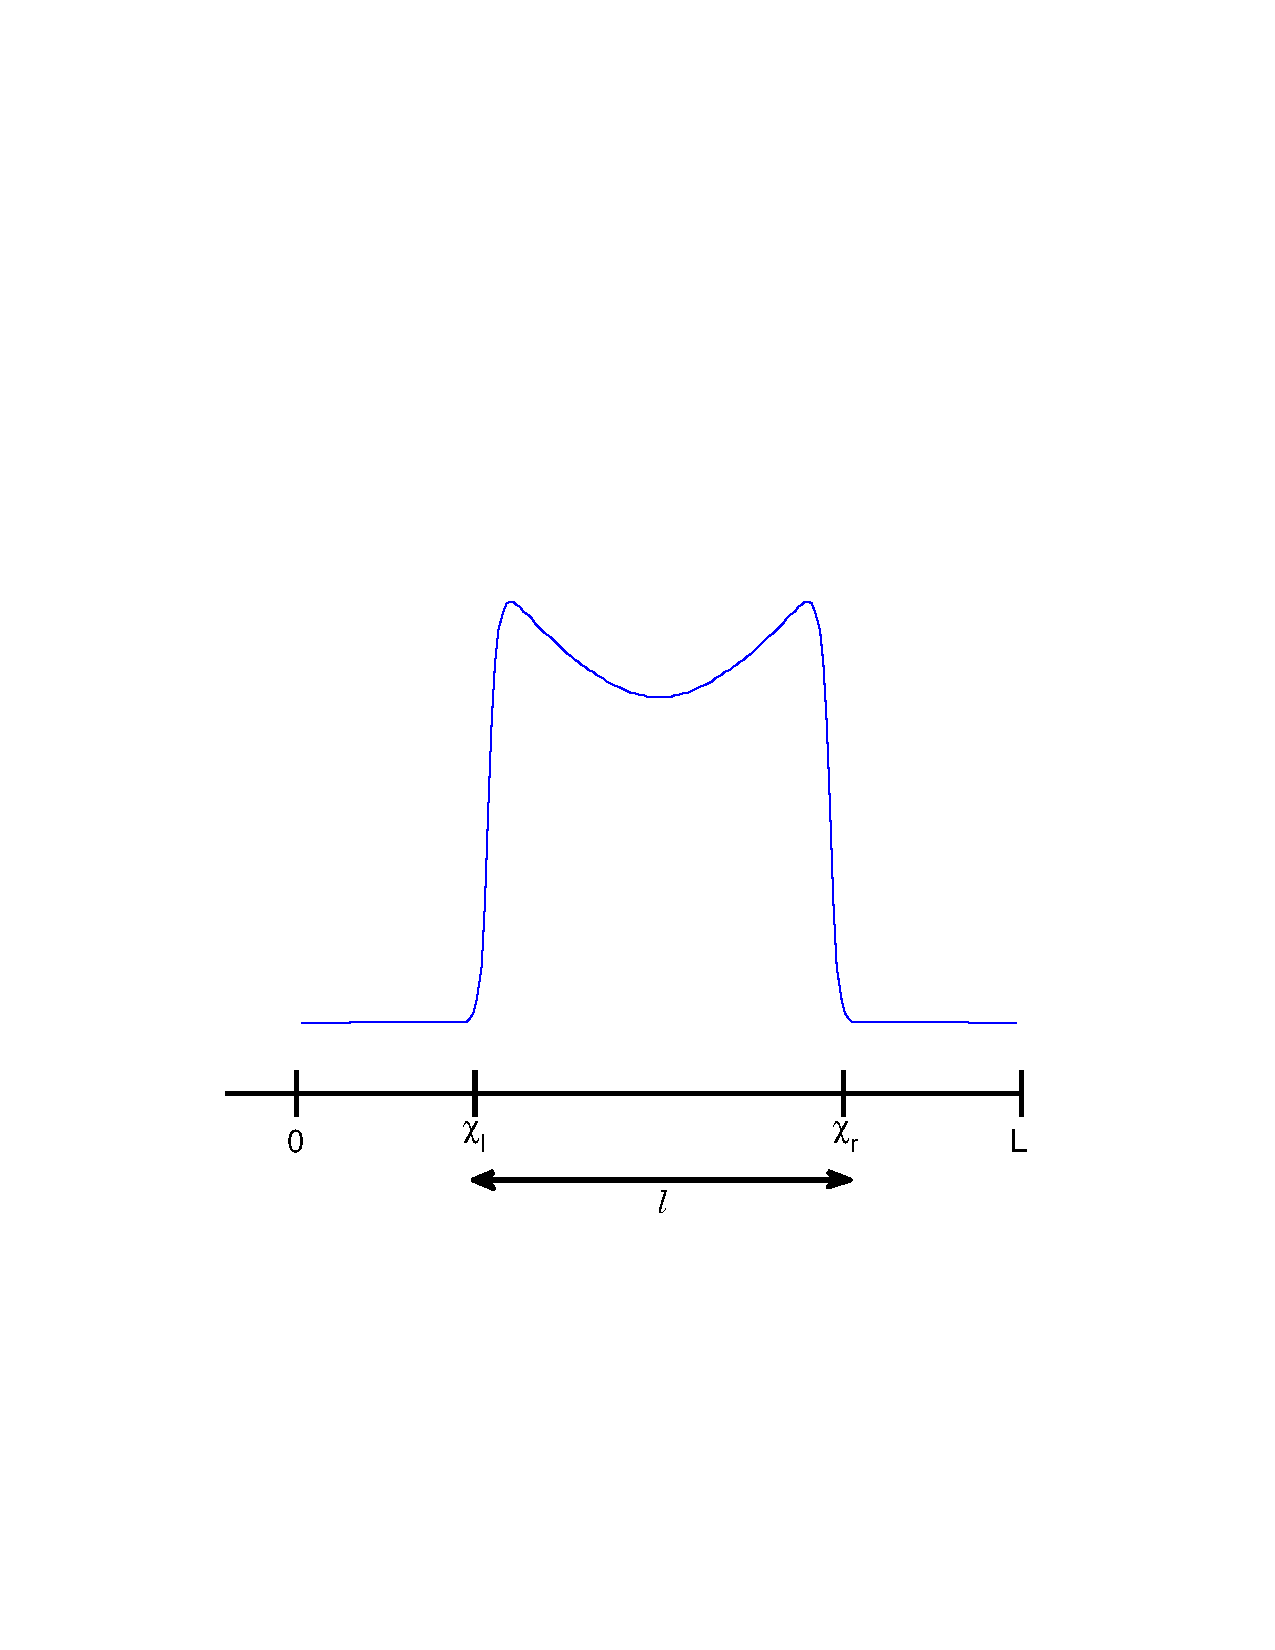
\includegraphics[width=4in]{single_mesa}
\caption{A typical mesa profile in the stationary solution $v(x)$. The left and right edges of the mesa are labelled as $\chi_l$ and $\chi_r$ respectively; and the length of the mesa section is $l$ (***add multi-mesa picture)) *** wrong fig.}
\label{fig:single_mesa}
\end{center}
\end{figure}
% 
The stationary equation we want to solve is
% 
\begin{equation}
\label{eqn:gms_stat}
\begin{split}
\begin{aligned}
	0 &= \Ep^2 u_{xx}+ f(u,v),\qquad &u_x(-L)=u_x(L)=0, \\
	0 &= \frac{\DD}{\Ep}v_{xx}+ g(u,v),\qquad &v_x(-L)=v_x(L)=0.
\end{aligned}
\end{split}
\end{equation}
% 
To first order, we have $v_{xx}=0$. Applying the Neumann boundary condition, we have then that $v\sim\VV$, and the value of the constant can be estimated by integrating over the whole domain. The resulting equation is	
% 
\begin{equation}
\label{eqn:v_first_order}
  0 = \int_0^Lg(u,\VV)dx,
\end{equation}
% 
with $v=\VV$ constant.

Now, we are looking for a heteroclinic connection in $u$ as the transition mechanism connecting $u=u_+$ to $u=u_-$. This imposes the algebraic constraint that $f(u_+,V)\equiv f_+ = 0$, and $ f(u_-,V) \equiv f_- = 0$, which has to be satisfied together with the Maxwell line condition \cite{maxwell1994} $\int_{u_-}^{u_+} f(w,\VV)dw = 0$. For both branches to be stable we also require $f_u(u_{\pm},\VV)<0$. Solving the algebraic system determines $u_{\pm}$, and $v_0=\VV$.

In the inner region near the interface of the mesa, we have that $v\sim\VV$, and we do a change of variables for $y=\Ep^{-1}(x-l)$, and $u(x)\sim U_0(\frac{x-l}{\Ep})$ . Integrating \eqref{eqn:v_first_order} in two parts across the interface yields the following result
% 
\begin{equation*}
\label{eqn:w_eqn}
\begin{split}
\begin{aligned}
  0 &= \frac{D}{\Ep}\int_0^lv_{xx}+\int_0^lg(u,\VV)dx\quad&\Rightarrow&\qquad \frac{D}{\Ep}v_x(l^-)=-lg_+,\\
  0 &= \frac{D}{\Ep}\int_l^Lv_{xx}+\int_l^Lg(u,\VV)dx\quad&\Rightarrow&\qquad \frac{D}{\Ep}v_x(l^+)=(L-l)g_-.
\end{aligned}
\end{split}
\end{equation*}

Since the $v$ solution doesn't have sharp interfaces, we have then that to first order
% 
\begin{equation}
\label{eqn:l_eqn}
\begin{split}
  l = \frac{g_-}{g_- - g_+}L + O(\Ep).
\begin{aligned}
\end{aligned}
\end{split}
\end{equation}
% 

Furthermore, since $0<l<L$, we have the consistency condition
% 
\begin{equation*}
  0<\frac{g_-}{g_- - g_+}<1,
\end{equation*}
% 
and as with $f_{\pm}$, we have that $g_{\pm} \equiv g(u_{\pm},\VV)$.

We will divide the half-mesa branch into three regions: the outer part on the mesa plateau, $0<x<l$; the outer part of the mesa beyond the plateau, $x>l$; and the internal layer around $x=l$ bridging the two outer regions.

To zoom into the inner layer we let $y=\frac{x-l}{\Ep},\hspace{1ex} u(\Ep y+l)\equiv U(y),\hspace{1ex} v(\Ep y+l)\equiv V(y)$; which when substituted into \eqref{eqn:gms_stat} results in
% 
\begin{equation}
\label{eqn:gms_layer}
\begin{split}
\begin{aligned}
	&U_{yy}+ f(U,V) =0,\qquad &\infty<y<\infty,\qquad &U\rightarrow U_{\pm} \text{ as } y\rightarrow\mp\infty,\\
	&V_{yy}+ \frac{\Ep^3}{\DD} g(U,V)=0,\qquad &\infty<y<\infty,\qquad &V\rightarrow V_{\pm} \text{ as } y\rightarrow\mp\infty.
\end{aligned}
\end{split}
\end{equation}
% 

In the outer region, $0<x<l$, we have
% 
\begin{equation*}
% \label{eqn:gms_outer1}
\begin{split}
\begin{aligned}
	&f(u,v) = 0,\qquad &u_x(0)=0,\\
	&v_{xx}+ \frac{\Ep}{\DD} g(u,v) = 0,\qquad &v_x(0)=0.
\end{aligned}
\end{split}
\end{equation*}
% 
with the boundary conditions stemming from the even symmetry imposed on the mesas. Similarly, for the region $x>l$ we have
% 
\begin{equation}
\label{eqn:gms_outer2}
\begin{split}
\begin{aligned}
	&f(u,v) = 0,\qquad &u_x(L)=0,\\
	&v_{xx} + \frac{\Ep}{\DD} g(u,v) = 0,\qquad &v_x(L)=0.
\end{aligned}
\end{split}
\end{equation}
% 

Performing an asymptotic expansion $u = u_- + \frac{\Ep}{\DD}u_1 + \cdots, \hspace{1ex} v = \VV + \frac{\Ep}{\DD}v_1 + \cdots$, and substituting into a Taylor expansion of $f(u,v)$ in \eqref{eqn:gms_outer2}, we obtain
% 
\begin{equation*}
% \label{eqn:taylor_f}
\begin{split}
\begin{aligned}
	&f(u_-,\VV) + \frac{\Ep}{\DD}(f_u^-u_1 + f_v^-v_1) + \cdots = 0,\\
\end{aligned}
\end{split}
\end{equation*}
%
thus $u_1 = -\frac{f_v^-}{f_u^-}v_1$, where $f_v^{\pm} = f_v(u_{\pm},\VV)$, and  $f_u^{\pm} = f_u(u_{\pm},\VV)$.

From \eqref{eqn:gms_outer2} we also obtain that
% 
\begin{equation}
\label{eqn:v_outer}
\begin{split}
\begin{aligned}
	&v_{1xx} = -g_-,\qquad\text{on }l<x<L,\qquad\text{with }g_- = g(u_-,\VV),\\
	&v_{1x}(L) = 0,\qquad v_1(l^+)=v_{1-},
\end{aligned}
\end{split}
\end{equation}
%
where we have imposed the boundary condition $v_1(l^+) = v_{1-}$ in terms of an unknown constant $v_{1-}$ to be calculated later.

The solution in this region is
% 
\begin{equation}
\label{eqn:v1}
\begin{split}
\begin{aligned}
	v_1(x) = -g_-\left(\frac{1}{2}(x-L)^2-\frac{1}{2}(L-l)^2\right) + v_{1-},
\end{aligned}
\end{split}
\end{equation}
%
therefore we have that in the outer region $l<x<L$ 
% 
\begin{equation}
\label{eqn:uv_outer2}
\begin{split}
\begin{aligned}
	&u\sim u_- + \frac{\Ep}{\DD}\left(-\frac{f_v^-}{g_u^-}v_1(x) \right),\\
	&v\sim \VV + \frac{\Ep}{\DD}v_1(x).
\end{aligned}
\end{split}
\end{equation}
%
Either by derivating \eqref{eqn:uv_outer2}, or integrating \eqref{eqn:v_outer} over $l<x<L$ we get that $v_{1x}(l^+)\equiv v_{1-}' = g_-(L-l)$.

An analogous calculation on the outer region $0<x<l$ yields 
% 
\begin{equation*}
% \label{eqn:uv_outer1}
\begin{split}
\begin{aligned}
	&u\sim u_+ + \frac{\Ep}{\DD}\left(-\frac{f_v^+}{g_u^+}v_1(x) \right),\\
	&v\sim \VV + \frac{\Ep}{\DD}v_1(x),\quad\text{with}\quad v_1(x) = -g_+\left(\frac{1}{2}x^2-\frac{l^2}{2} \right) + v_{1+},
\end{aligned}
\end{split}
\end{equation*}
%
again with a boundary condition $v_1(l^-)=v_{1+}$ in terms of an unknown constant to be found. 

% 
\begin{equation}
\label{eqn:matching_inner}
\begin{split}
\begin{aligned}
	v_{1x}(l^-)\equiv v_{1+}' &= -g_+l,\\
	v_{1x}(l^+)\equiv v_{1-}' &= g_-(L-l).
\end{aligned}
\end{split}
\end{equation}
%

Taylor expanding both solutions near $x=l^{\pm}$ provides matching conditions for the inner solution. The problem for the inner layer, in terms of the variable $y=\Ep^{-1}(x-l)$, is
% 
\begin{equation*}
% \label{eqn:uv_inner2}
\begin{split}
\begin{aligned}
	&U_{yy}+f(U,V)=0,\quad -\infty<y<\infty,\quad U\sim u_{\pm}-\frac{\Ep}{\DD}\frac{f_v^{\pm}}{f_u^{\pm}}v_{1\pm}\text{ as }y\rightarrow\mp\infty ,\\
	&V_{yy}=-\frac{\Ep^3}{\DD}g(U,V),\quad -\infty<y<\infty,\quad V\sim \VV+\frac{\Ep}{\DD}(V_{1\pm}+\Ep yV_{1\pm}') \text{ as }y\rightarrow\mp\infty.
\end{aligned}
\end{split}
\end{equation*}
%

Expanding the inner solution, $U = U_0 + \frac{\Ep}{\DD}U_1 + \cdots,\hspace{1ex} V = V_0 + \frac{\Ep}{\DD}V_1 + \cdots$, we get
% 
\begin{equation*}
% \label{eqn:uv_inner1}
\begin{split}
\begin{aligned}
	\LL(U_1) &= U_{1yy}+f_U(U_0,V_0)U_1=-f_V(U_0,V_0)V_1,\\
	V_{1yy} &= 0.
\end{aligned}
\end{split}
\end{equation*}
%

The matching condition for $V_1 = h_1y+h_2$ is $V_1\sim v_{1\pm}\text{ as }y\rightarrow\mp\infty$. Thus we must have that $h_1=0$, and $h_2 = v_{1+} = v_{1-} = V_1$.

We can obtain a solvability condition since by translational invariance we have that $\LL(U_0') = 0$. Hence
% 
\begin{equation*}
% \label{eqn:solva1}
\begin{split}
\begin{aligned}
	\int_{-\infty}^{\infty}(U_0'\LL U_1 - U_1\LL U_0')dy = -V_1\int_{-\infty}^{\infty}U_0'f_V(U_0,V_0)dy = 0.
\end{aligned}
\end{split}
\end{equation*}
%

We can conclude then that if $f_V\neq0$ then $V_1=0$, thus $V_{1\pm}=0$. We also have then that $U_1 = cU_0'$, and without loss of generality we take $c=0$.

To $O(\Ep)$ we have then
% 
\begin{equation}
\label{eqn:u_outer}
	\begin{split}
	v(x) &= \left\{
	\begin{matrix}
	  \VV + \frac{\Ep}{2\DD}\left(g_-(x-L)^2 + g_-(L-l)^2 \right),&l<x<L,\\
	  \VV - \frac{\Ep}{2\DD}g_+(x^2-l^2),\hspace{1in}&0<x<l.
	\end{matrix}\right.\\
	u(x) &= \left\{
	\begin{matrix}
	  u_- + O(\frac{\Ep^2}{\DD}),\hspace{1.43in}&l<x<L,\\
	  u_+ + O(\frac{\Ep^2}{\DD}),\hspace{1.42in} &0<x<l.
	\end{matrix}\right.\\
	\end{split}
\end{equation}
% 

In the inner region we expand to second order, $u=U_0 + \frac{\Ep^2}{\DD}U_2+\cdots,\hspace{1ex}, v = \VV + \frac{\Ep^2}{\DD}V_2+\cdots$, and get
% 
\begin{equation*}
% \label{eqn:uv_inner_O2}
\begin{split}
\begin{aligned}
	\LL(U_2) &= U_{2yy}+f_U(U_0,V_0)U_2=-f_V(U_0,V_0)V_2,\\
	V_{2yy} &= 0,
\end{aligned}
\end{split}
\end{equation*}
%
with the matching condition that $V_2\sim yv_{1\pm}'\text{ as }y\rightarrow\mp\infty$, and $v_1$ the $O(\Ep/\DD)$ term for $v(x)$ in \eqref{eqn:u_outer}.

We must have then that $V_2(y) = H_{20} + yH_{21}$, and we can conclude that $H_{21} = V_{1+}' = V_{1-}'$. Using \eqref{eqn:matching_inner}, we can now recover the result from \eqref{eqn:l_eqn}:
% 
\begin{equation*}
	g_-(L-l) = -g_+l\qquad \rightarrow \qquad l=\frac{g_-}{g_- - g_+}L.
\end{equation*}
% 

The constant $H_{20}$ can be found in terms of $H_{21}$ via a solvability condition, since $\LL U_0' = 0$, and 
% 
\begin{equation*}
	\LL U_2 = U_{2yy} + f_U(U_0,V_0)U_2 = -f_V(U_0,V_0)(H_{20}+yH_{21}),\\
\end{equation*}
% 

We have then that
% 
\begin{equation*}
\begin{split}
\begin{aligned}
  \int_{-\infty}^{\infty}(H_{20}+yH_{21})U_0'f_V(U_0,V_0)dy = 0,\\
	\text{hence}\quad H_{20} = -V_{1\pm}'\frac{\int_{-\infty}^{\infty}yU_0'f_V(U_0,V_0)dy}{\int_{-\infty}^{\infty}U_0'f_V(U_0,V_0)dy}
\end{aligned}
\end{split}
\end{equation*}
% 

In the outer expansion, $v(x) = \VV + \frac{\Ep}{\DD}v_1 + \frac{\Ep^2}{\DD}v_2$, we require then that $v_2(l) = H_{20}$.


\subsection{Stability of the solution to perturbations along the y-axis}


We start by considering a one-mesa steady-state solution to the domain $[-L,L]\times[0,d_0]$. We consider small perturbations of the form
% 
\begin{equation*}
% \label{eqn:pert}
\begin{split}
\begin{aligned}
  u(x,y) &= u_e(x) + e^{\lA t}e^{imy}\phi(x),\\
  v(x,y) &= v_e(x) + e^{\lA t}e^{imy}\psi(x),
\end{aligned}
\end{split}
\end{equation*}
% 
which yield the eigenvalue problem
% 
\begin{equation}
\label{eqn:eigen_uv}
\begin{split}
  \lA \phi &= \Ep^2\phi_{xx} - \Ep^2m^2\phi + f_u(u_e,v_e)\phi + f_v(u_e,v_e)\psi,\\
  \tau\lA \psi &= \frac{\DD}{\Ep}\psi_{xx} - \frac{\DD}{\Ep}m^2\psi + g_u(u_e,v_e)\phi + g_v(u_e,v_e)\psi.
\end{split}
\end{equation}
% 


We now multiply the $\phi$ equation in \eqref{eqn:eigen_uv} by $u_x$ and integrating by parts on $[0,L]$. Given that the equilibrium problem satisfies $\Ep^2u_{xx} + f(u,v) = 0$, we have then that
% 
\begin{equation*}
% \label{eqn:operator_u}
\begin{aligned}
	\Ep^2(u_x)_{xx} + f_uu_x + f_vv_x = 0.
\end{aligned}
\end{equation*}
% 

We define the operator $\LL_{\Ep}u$ by
% 
\begin{equation*}
   \LL_{\Ep}u\equiv \Ep^2u_{xx} + f_u u,
\end{equation*}
% 
and we have then that the equilibrium problem satisfies
% 
\[
   \LL_{\Ep}u_x = \Ep^2(u_x)_{xx} + f_u u_x = -f_v v_x,
\]
% 
and from \eqref{eqn:eigen_uv} we have then that
% 
\[
   \LL_{\Ep}\phi +f_v\psi = \bar{\lA}\phi.
\]
% 

Integrating first on $-L<x<0$, we have
% 
\[
 \int_{-L}^0(u_x\LL_{\Ep}\phi - \phi\LL_{\Ep}u_x)dx = \Big.\Ep^2[u_x\phi_x-\phi u_{xx}]\Big|_{-L}^0.
\]
%  

The two terms on the left side of the integral each equate to
% 
\begin{equation*}
\begin{split}
	\int_{-L}^0u_x\LL_{\Ep}\phi dx &= \bar{\lA}\int_{-L}^0u_x\phi dx - \int_{-L}^0u_xf_v\psi dx\\
	\int_{-L}^0\phi\LL_{\Ep}u_x dx &= -\int_{-L}^0\phi f_vv_x.
\end{split}
\end{equation*}
% 

Putting it all together leads to 
% 
\[
  \bar{\lA}\int_{-L}^0u_x\phi dx - \int_{-L}^0u_xf_v\psi dx + \int_{-L}^0\phi f_vv_x = \Big.\Ep^2[u_x\phi_x-\phi u_{xx}]\Big|_{-L}^0.
\]
% 

We now make use of the following facts: $u_x(-L)=u_x(0)=0$ from Neumann boundary conditions and even symmetry considerations, respectively. Both $\psi(x)$ and $v_x(x)$ are approximately constant, hence $\psi(x)\cong \psi(-l)$, $v_x(x)\cong v_x(-l)$. Since $u_x(x)$ is localized near the interface, we have that 
% 
\[
  \int_{-L}^0u_x\phi dx = c_-\int_{-L}^0u_x^2dx.
\]
% 

This reduces the equation to
% 
\begin{equation*}
\begin{split}
	\bar{\lA}c_-\int_{-L}^0u_x^2 dx &\cong \psi(-l)\int_{-L}^0u_xf_vdx - v_x(-l)c_-\int_{-L}^0f_vu_xdx - \Big.\Ep^2[\phi u_{xx}]\Big|_{-L}^0,\\
	\bar{\lA}c_-\int_{-L}^0u_x^2 dx &\cong \left[\psi(-l) - v_x(-l)c_-\right]\int_{-L}^0u_xf_vdx - \Big.\Ep^2[\phi u_{xx}]\Big|_{-L}^0,
\end{split}
\end{equation*}
% 

We now estimate 
% 
\begin{equation*}
\begin{split}
\begin{aligned}
\Big.\phi \Big|_{x=-L} &= O(1),\qquad \Big.\phi \Big|_{x=0} = O(1), \text{ as well as} \\
\Big.u_{xx} \Big|_{x=-L} &= O(\Ep), \quad\Big.u_{xx} \Big|_{x=0} = O(\Ep),
\end{aligned}
\end{split}
\end{equation*}
% 
therefore we have that $\Big.\Ep^2(\phi u_{xx})\Big|_{-L}^0 = O(\Ep^3)$.

Changing variables to $y = \Ep^{-1}(x+l)$, we have that
% 
\begin{equation*}
\begin{split}
	\int_{-L}^0u_xf_vdx\sim \int_{-\infty}^{\infty}U_0'(y)f_vdy = \int_{u_-}^{u_+}f_vdu,
\end{split}
\end{equation*}
% 
since $u\rightarrow u_{\pm}$ when $y\rightarrow\pm\infty$. Similarly, we can make the same change of variables to have
% 
\begin{equation*}
\begin{split}
	\int_{-L}^0u_x^2dx\sim \int_{-L}^{0}\frac{1}{\Ep^2}(U_0')^2dx = \frac{1}{\Ep}\int_{-\infty}^{\infty}(U_0')^2dy.
\end{split}
\end{equation*}
% 

This yields the simplified equation
% 
\begin{equation*}
\begin{split}
	\bar{\lA}c_-\int_{-\infty}^{\infty}(U_0')^2 dy \sim \Ep\left[\psi(-l) - c_-v_x(-l)\right]\int_{u_-}^{u_+}f_vdu + O(\Ep^4).
\end{split}
\end{equation*}
% 

We now define 
% 
\begin{equation*}
\begin{split}
	\kA_0 \equiv \frac{\int_{-\infty}^{\infty}(U_0')^2 dy}{\int_{u_-}^{u_+}f_vdu}.
\end{split}
\end{equation*}
% 

The integral in the denominator, $\int_{-\infty}^{\infty}(U_0')^2dy$, can be further estimated by integrating the $U$ equation in \eqref{eqn:gms_layer}
% 
\begin{equation*}
\label{eqn:beta}
\begin{split}
  \int_{-\infty}^{\infty}U_{0y}^2(y)dy \sim \int_{0}^{u_+}U_{0y}^2\frac{1}{U_{0y}}dU_0 = \int_0^{u_+}\sqrt{2\FF(u)}du,
\end{split}
\end{equation*}
% 
with $\FF(u)=-\int_0^uf(s)ds$.


then, 
% 
\begin{equation*}
\begin{split}
	\bar{\lA}\kA_0c_-\sim\Ep\left[\psi(-l) - v_x(-l)c_-\right]
\end{split}
\end{equation*}
% 

Repeating the procedure for the $0<x<L$ region, we get the analogous equation
% 
\begin{equation*}
\begin{split}
	\bar{\lA}\kA_0c_+\sim\Ep\left[-\psi(l) + v_x(l)c_+\right],
\end{split}
\end{equation*}
% 
with the sign change from the fact that with a change of variables $y=\Ep^{-1}(x-l)$ and the transition layer at $x=l$, in this region we have $u\rightarrow u_{\pm}$ when $y\rightarrow\mp\infty$.

We recall from \eqref{eqn:v1} and \eqref{eqn:uv_outer2} that $v_x(l) \sim \frac{\Ep}{\DD}g_-(L-l)$, 
and we also know from \eqref{eqn:l_eqn} that $l = \frac{g_-L}{g_--g_+}$, therefore
% 
\begin{equation*}
\begin{split}
	v_x(l) = -\left(\frac{\Ep}{\DD}\right)\frac{g_-g_+L}{g_--g_+}.
\end{split}
\end{equation*}
% 

Furthermore, since $v(x)$ is an even function, we have that $v_x(-l) = -v_x(l)$.

We can collect both equations into the following linear system
% 
\begin{equation}
\label{eqn:lam}
	\begin{split}
	\Ep^{-1}\bar{\lA}\kA_0\begin{pmatrix}c_+\\c_-\end{pmatrix}
   &\cong
	\begin{pmatrix} -\psi(l) \\ \psi(-l) \end{pmatrix}
	 +v_x(l) \begin{pmatrix}c_+\\c_-\end{pmatrix}\\
   &\cong
	\begin{pmatrix} -\psi(l) \\ \psi(-l) \end{pmatrix}
	 - \left(\frac{\Ep}{\DD}\right)\frac{g_-g_+L}{g_--g_+}
	\begin{pmatrix}c_+\\c_-\end{pmatrix}
	\end{split}
\end{equation}
% 
\begin{remark}
The goal at this point is to find $\lA$; to establish the conditions under which the system is linearly stable or unstable it is sufficient to determine the sign of $\lA$. To fully solve the system in \eqref{eqn:lam} we need to find $\psi(\pm l)$, and this has to be done by finding the equilibrium solution for the second equation in \eqref{eqn:eigen_uv}:
% 
\begin{equation}
\label{eqn:psi_eq}
\begin{split}
	\psi_{xx} - m^2\psi + \frac{\Ep}{\DD}(g_u\phi + g_v\psi)=0.
\end{split}
\end{equation}
% 
\end{remark}

At this point we can take into account the possibility that the solution might consist of $k-$mesas. The one mesa problem in $-L<x<L$ can be extended to the $K-$mesa case on $-L<x<(2K-1)L$ by means of Floquet theory. This can be accomplished for the $\psi$ equation by using the following boundary conditions:
% 
\begin{equation*}
  \psi(L) = z\psi(-L),  \psi'(L) = z\psi'(-L).
\end{equation*}
% 

The system \eqref{eqn:eigen_uv} can then be extended to the interval $[L,3L]$ defining $\phi(x):=z\phi(x-2L)$ and similarly for $\psi$. At the boundary we have that $\phi(3L) = z^2\phi(L)$. This can be repeated $K$ times, and we have that the boundary of the whole interval $[-L,(2K-1)L]$ satisfies $\phi(2KL-L) = z^K\phi(-L)$ (similarly for $\psi$). We can get standard periodic boundary conditions then by simply choosing $z = e^{2\pi ik/K},\quad k = 0,\hdots,K-1$. 

Do note that this is not quite the same as having homogeneous Neumann boundary conditions as in the original problem. However, performing a horizontal reflection of such a solution results in a smooth periodic boundary solution. Reversing this procedure allows us to use the periodic boundary solution to construct the desired homogeneous Neumann; this results in having to consider $2K$ mesas in the periodic case, and thus having $z = e^{2\pi ik/2K},\quad k = 0,\hdots,K-1$.

Since $u(x)$ is approximately constant except at the interfaces, we can approximate the eigenfunction $\phi\sim c_{\pm}u_x$, and similarly $\psi\sim\psi(\pm l)$ when $x\sim\pm l$.

In the flat regions $|x|<l$ and $l<|x|<L$ we have that 	$f_u\phi + f_v\psi = \lA\phi$. We will show later that $\lA\ll 1$, and this can be used to approximate
% 
\begin{equation*}
\begin{split}
	\phi&\sim -\frac{f_v^+}{f_u^+}\psi\qquad\text{for }|x|<l,\\
	\phi&\sim -\frac{f_v^-}{f_u^-}\psi\qquad\text{for }l<|x|<L.
\end{split}
\end{equation*}
% 

Substituting it into \eqref{eqn:psi_eq}, we end up with the ODE
% 
\begin{equation}
\label{eqn:psi_aprox}
\begin{split}
	\psi_{xx} - \sI_{\pm}^2\psi = 0,
\end{split}
\end{equation}
% 
which is defined everywhere except at the interfaces, and where
% 
\begin{equation*}
% \label{eqn:psi_aprox1}
\begin{split}
	&\quad\sI_{\pm}^2 = m^2  + \frac{\Ep}{\DD}\kA_{\pm} + \frac{\Ep\tau\lA}{\DD}, \text{ with}\\
	\kA_+ &\equiv - \left(g_v^+ - \frac{f_v^+}{f_u^+}g_u^+ \right)>0,\qquad \text{when }|x|<l \\
	\kA_- &\equiv - \left(g_v^- - \frac{f_v^-}{f_u^-}g_u^- \right)>0,\qquad \text{when }l<|x|<L,
\end{split}
\end{equation*}
% 
and as before, we are using the notation $f_v^+\equiv \pAr vf(u^+,\VV)$.

\begin{remark}
	We will eventually show that for $m\neq0$ we have that $\lA=O(\Ep^2)$, and that $\lA=O(\Ep)$ for $m=0$. It is tempting to disregard the $\tau\lA\Ep$ term in \eqref{eqn:eigen_uv}, however, we will keep this term in order to analyze the case when $\tau\rightarrow\infty$.
\end{remark}

Since $\psi$ is smooth, the jump across $x=\pm l$ can be estimated in the sense of distributions through the term $g_u\phi$. We start with the jump across $x=l$, with the standard inner change of variables $y=\Ep^{-1}(x-l)$,
% 
\begin{equation*}
% \label{eqn:phi_aprox1}
\begin{split}
	g_u\phi\sim g_u c_+u_x\rightarrow c_+\int_{l^-}^{l^+}g_uu_xdx 
	&\sim c_+\int_{-\infty}^{+\infty}g_{U_0}U_{0y}dy \\
	&\sim c_+\int_{u_+}^{u_-}g_{U_0}dU_0\sim c_+(g_- - g_+).
\end{split}
\end{equation*}
% 

Similarly, for the jump across $x=-l$, with $y=\Ep^{-1}(x+l)$, we have
% 
\begin{equation*}
% \label{eqn:phi_aprox2}
\begin{split}
	g_u\phi\sim g_u c_-u_x\rightarrow c_-\int_{-l^+}^{-l^-}g_uu_xdx 
	&\sim c_-\int_{-\infty}^{+\infty}g_{U_0}U_{0y}dy \\
	&\sim c_-\int_{u_-}^{u_+}g_{U_0}dU_0\sim c_-(g_+ - g_-).
\end{split}
\end{equation*}
% 

Therefore, we have
% 
\begin{equation*}
% \label{eqn:phi_aprox3}
\begin{split}
	g_u\phi\sim c_+(g_- - g_+)\dE(x-l) + c_-(g_+ - g_-)\dE(x+l),
\end{split}
\end{equation*}
% 
effectively taking into account the contributions from both interfaces.

We can now write \eqref{eqn:psi_aprox} defined on the whole interval $-L<x<L$ as
% 
\begin{equation*}
% \label{eqn:psi_aprox2}
\begin{split}
	\psi_{xx} - \sI_{\pm}^2\psi = \frac{\Ep}{\DD}(g_- - g_+)\big[c_+\dE(x-l) - c_-\dE(x+l)\big],
\end{split}
\end{equation*}
% 
with the added conditions that the solution has to be continuous across the interfaces at $x=\pm l$; that the jump conditions $\Big.\psi_x\Big|_{-l^-}^{-l^+} = c_-s$, and $\Big.\psi_x\Big|_{l^+}^{l^-} = c_+s$ are satisfied; and that the Floquet boundary conditions $\psi(L) = z\psi(-L)$, and $\psi'(L) = z\psi'(-L)$ are satisfied as well. 

For the jump conditions we have $s = \frac{\Ep}{\DD}(g_--g_+)$

A solution to the system with prescribed continuity across the interfaces is
% 
\begin{equation*}
% \label{eqn:psi_full}
	\begin{split}
	\psi(x) &= \left\{
	\begin{matrix}
	  \psi(-l)\dfrac{\cosh[\sI_-(x+L)]}{\cosh[\sI_-(L-l)]} + A_L\sinh[\sI_-(x+l)],&-L<x<l,\\
	  \psi(-l)\dfrac{\sinh[\sI_+(l-x)]}{\cosh(2\sI_+l)} + \psi(l)\dfrac{\sinh[\sI_+(x+L)]}{\sinh(2\sI_+l)},&-l<x<l,\\
	  \psi(l)\dfrac{\cosh[\sI_-(L-x)]}{\cosh[\sI_-(L-l)]} + A_R\sinh[\sI_-(x-l)],&l<x<L,\\
	\end{matrix}\right.
	\end{split}
\end{equation*}
% 
the four unknowns $A_L, A_R, \psi(l), \psi(-l)$ can be determining by enforcing all four boundary and jump conditions.

We start with the Floquet boundary conditions. The four relevant terms are
% 
\begin{equation*}
\begin{split}
\begin{aligned}
	\psi(L) &= \frac{\psi(l)}{\cosh[\sI_-(L-l)]} + A_R\sinh[\sI_-(L-l)],\\
	z\psi(-L) &= \frac{z\psi(-l)}{\cosh[\sI_-(L-l)]} - zA_L\sinh[\sI_-(L-l)],\\
	\psi'(L) &= A_R\sI_-\cosh[\sI_-(L-l)],\\
	z\psi'(-L) &= zA_L\sI_-\cosh[\sI_-(L-l)].\\
\end{aligned}
\end{split}
\end{equation*}
% 

From the condition on $\psi'(L) = z\psi'(-L)$, it can immediately be seen that $zA_L = A_R$.

From the condition that $\psi(L) = z\psi(-L)$, we get
% 
\begin{equation*}
\begin{split}
	\frac{\psi(l)-z\psi(-l)}{\cosh[\sI_-(L-l)]} = -2zA_L\sinh[\sI_-(L-l)],
\end{split}
\end{equation*}
% 
hence
% 
\begin{equation}
\label{eqn:floquet1}
\begin{split}
	\psi(l)-z\psi(-l) = -zA_L\sinh[2\sI_-(L-l)]
\end{split}
\end{equation}
% 

For the jump conditions, the four relevant terms are
% 
\begin{equation*}
\begin{split}
\begin{aligned}
	\psi_x(l^+) &= -\psi(l)\sI_-\tanh[\sI_-(L-l)] + A_R\sI_-,\\
	\psi_x(l^-) &=  \psi(l)\sI_+\coth(2\sI_+l) - \psi(-l)\sI_+\csch(2\sI_+l),\\
	\psi_x(-l^+) &= \psi(l)\sI_+\csch(2\sI_+l) - \psi(-l)\sI_+\coth(2\sI_+l),\\
	\psi_x(-l^-) &= c,\\
\end{aligned}
\end{split}
\end{equation*}
% 

The two jump conditions, $\psi(l^+) - \psi(l^-) = c_+s$ and $\psi(-l^-) - \psi(-l^+) = c_-s$, yield
% 
\begin{equation*}
\begin{split}
\begin{aligned}
	& -\psi(l)\sI_-\tanh[\sI_-(L-l)] + A_R\sI_- - \\
	 & \qquad\qquad \psi(l)\sI_+\coth(2\sI_+l) + \psi(-l)\sI_+\csch(2\sI_+l) = c_+s,\\
	&\psi(-l)\sI_-\tanh[\sI_-(L-l)] + A_L\sI_- -  \\
	 & \qquad\qquad \psi(l)\sI_+\csch(2\sI_+l) + \psi(-l)\sI_+\coth(2\sI_+l) = c_-s
\end{aligned}
\end{split}
\end{equation*}
% 

Simplifying things slightly, and using $A_R = zA_L$, we get
% 
\begin{equation}
\label{eqn:psii}
\begin{split}
\begin{aligned}
	& -\psi(l)\big(\sI_-\tanh[\sI_-(L-l)] + \sI_+\coth(2\sI_+l) \big) + \psi(-l)\sI_+\csch(2\sI_+l) = c_+s - zA_L\sI_-,\\
	& -\psi(l)\sI_+\csch(2\sI_+l) + \psi(-l)\big(\sI_-\tanh[\sI_-(L-l)] + \sI_+\coth(2\sI_+l)\big)  = c_-s - A_L\sI_-
\end{aligned}
\end{split}
\end{equation}
% 

Putting together \eqref{eqn:psii} and \eqref{eqn:floquet1}, we can express $\psi(\pm l)$ as the solution to the linear system
% 
\begin{equation*}
% \label{eqn:lam}
	\begin{split}
	\begin{pmatrix} d&e\\e&d\end{pmatrix}
	\begin{pmatrix} \psi(l)\\ -\psi(-l)\end{pmatrix}
   &=
	-s\begin{pmatrix} c_+ \\ c_- \end{pmatrix}
	 +\sI_-A_L \begin{pmatrix}z\\1\end{pmatrix},\\
	\begin{pmatrix} z\\ 1\end{pmatrix}^T
  \begin{pmatrix} \psi(l)\\ -\psi(-l)\end{pmatrix} &= -A_Lz\sinh[2\sI_-(L-l)]
	\end{split}
\end{equation*}
% 
with 
% 
\[
\begin{split}
  d&\equiv \sI_-\tanh[\sI_-(L-l)] + \sI_+\coth(2\sI_+l),\\
  e&\equiv \sI_+\csch(2\sI_+l).
\end{split}
\]
% 

Solving for $A_L$ in the second equation, and substituting it into the first one yields
% 
\begin{equation*}
  G\vec{r} = -s\vec{c} + \vec{b}_0\left(\frac{-\vec{b}_1^T\vec{r}}{z\chi}\right),
\end{equation*}
% 
with 
% 
\begin{equation*}
% \label{eqn:lam}
	\begin{split}
	\begin{aligned}
	&G = \begin{pmatrix} d&e\\e&d\end{pmatrix},
	&&r = \begin{pmatrix} \psi(l)\\ -\psi(-l)\end{pmatrix},
	&&c = \begin{pmatrix} c_+\\ c_-\end{pmatrix},\\
	&\vec{b}_0 = \begin{pmatrix} z\\ 1\end{pmatrix},
	&&\vec{b}_1 = \begin{pmatrix} 1\\ z\end{pmatrix},
	&&\chi = \frac{\sinh[2\sI_-(L-l)]}{\sI_-}.
	\end{aligned}
	\end{split}
\end{equation*}
% 
This yields the matrix problem
% 
\begin{equation}
\label{eqn:reqn1}
  (G+B)\vec{r} = -s\vec{c},
\end{equation}
% 
where 
% 
\[
  B = \frac{1}{z\chi}\vec{b}_0\vec{b}_1^T = \frac{1}{z\chi}\begin{pmatrix} z&z^2\\1& z\end{pmatrix} =
  \frac{1}{\chi}\begin{pmatrix} 1&z\\ \bar{z}& 1\end{pmatrix},
\]
% 
since $z\bar{z}=1$.

Recall that the eigenvalue system that we want to solve, from \eqref{eqn:lam}, is
% 
\begin{equation*}
% \label{eqn:lam}
	\begin{split}
	\Ep^{-1}\bar{\lA}\kA_0\begin{pmatrix}c_+\\c_-\end{pmatrix}
   &=
	\begin{pmatrix} -\psi(l) \\ \psi(-l) \end{pmatrix}
	 +v_x(l) \begin{pmatrix}c_+\\c_-\end{pmatrix},
	\end{split}
\end{equation*}
%
or, using compact notation
% 
\begin{equation}
\label{eqn:reqn2}
 \Ep^{-1}\bar{\lA}\kA_0\vec{c} = \vec{r} + v_x(l)\vec{c}.
\end{equation}
% 

Solving for $\vec{r}$ in \eqref{eqn:reqn1}, and substituting into \eqref{eqn:reqn2} yields
% 
\begin{equation}
\label{eqn:reqn3}
 \frac{\Ep^{-1}\bar{\lA}\kA_0}{s}\vec{c} = (G+B)^{-1}\vec{c} + \frac{v_x(l)}{s}\vec{c}.
\end{equation}
% 

Now, 
% 
\[
  \frac{v_x(l)}{s} = -\frac{\Ep}{\DD}\frac{g_-g_+L}{g_--g_+}\frac{\DD}{\Ep(g_+-g_-)} = \frac{g_-g_+L}{(g_+-g_-)^2}.
\]
% 

Since 
% 
\[
  l=\frac{g_-}{g_--g_+}L\qquad\rightarrow\qquad\frac{g_+}{g_-} = 1-\frac{L}{l},
\]
% 
we can then calculate
% 
\[
  \frac{v_x(l)}{s} = \frac{l^2}{L}\left(1-\frac{L}{l} \right) = \left(1-\frac{L}{l} \right)\frac{l^2}{L^2}L.
\]
% 

Similarly,
% 
\[
  \frac{\Ep^{-1}\bar{\lA}\kA_0}{s} = \frac{\Ep^{-1}\bar{\lA}\kA_0}{\Ep(g_+-g_-)/\DD} = -\frac{\DD}{\Ep^2}\frac{\bar{\lA}\kA_0}{g_-}\frac{l}{L}.
\]
% 

Substituting into \eqref{eqn:reqn3}, with $\bar{\lA} = \lA + \Ep^2m^2$, we obtain
% 
\begin{equation}
\label{eqn:ceqn1}
(G+B)^{-1}\vec{c} + \left(1- \frac{L}{l}\right)\frac{l^2}{L^2}L\vec{c} - m^2\vA\bar{c} = \frac{\vA}{\Ep^2}\lA\bar{c},
\end{equation}
% 
with $\vA = -\frac{\DD}{g_-}\kA_0\left(\frac{l}{L} \right)$.

The eigenpairs $\lA$ and $\bar{c}$ of \eqref{eqn:ceqn1} are given in terms of the spectrum of the two-by-two matrix $(G+B)^{-1}$, 
% 
\[
 (G+B)^{-1}\vec{\nu}_{\pm} = \omega_{\pm}\vec{\nu}_{\pm},
\]
% 
they are given as
% 
\begin{equation}
\label{eqn:lam2}
	\begin{split}
	\begin{aligned}
	  \vec{c} &= \vec{\nu}_+,\qquad\text{and}\qquad \lA_+ = \frac{\Ep^2}{\vA}\left[\omega_+ + \left(1- \frac{L}{l}\right)\frac{l^2}{L^2}L - m^2\vA \right],\\
	  \vec{c} &= \vec{\nu}_-,\qquad\text{and}\qquad \lA_- = \frac{\Ep^2}{\vA}\left[\omega_- + \left(1- \frac{L}{l}\right)\frac{l^2}{L^2}L - m^2\vA \right].
	\end{aligned}
	\end{split}
\end{equation}
%

This will yield two eigenpairs for each value of $z$. Thus we only need to find the spectrum of $(G+B)^{-1}$, and this can be done by first calculating the eigenpairs of $G+B$, and then taking the reciprocals of the eigenvalues.

Since the matrix
% 
\[
  G+B = \begin{pmatrix}d&e\\e&d\end{pmatrix} + \frac{1}{\chi}\begin{pmatrix}1&z\\ \bar{z}&1\end{pmatrix}
\]
% 
is a Hermitian matrix, then all the eigenvalues must be real, and it is possible to find an orthonormal basis.

We let $(G+B)\vec{\nu}=\sI\vec{\nu}$, and we have
% 
\[
  \det\begin{pmatrix} d+\frac{1}{\chi}-\sI&e+\frac{z}{\chi}\\ e+\frac{\bar{z}}{\chi}&d+\frac{1}{\chi}-\sI\end{pmatrix}=0.
\]
% 

Thus
% 
\begin{equation*}
% \label{eqn:lam2}
	\begin{split}
		\left(d+\frac{1}{\chi}-\sI \right)^2 &= \left(e+\frac{z}{\chi} \right)\left(e+\frac{\bar{z}}{\chi} \right),\\
		&= e^2 + \frac{1}{\chi^2} + \frac{e}{\chi}(z+\bar{z}),
	\end{split}
\end{equation*}
%
and we have used the fact that $z\bar{z}=1$.

Thus
% 
\begin{equation*}
% \label{eqn:lam2}
	\begin{split}
		d+\frac{1}{\chi}-\sI =\pm\left( e^2 + \frac{1}{\chi^2} + \frac{2e}{\chi}\mathrm{Re}(z)\right)^{1/2},
	\end{split}
\end{equation*}
%
and we can conclude that the eigenvalues of $(G+B)^{-1}$, needed in \eqref{eqn:lam2}, are simply
% 
\begin{equation*}
% \label{eqn:lam3}
	\begin{split}
	  \omega_{\pm} = \frac{1}{d+\frac{1}{\chi}\pm\left( e^2 + \frac{1}{\chi^2} + \frac{2e}{\chi}\mathrm{Re}(z)\right)^{1/2}}.
	\end{split}
\end{equation*}
%

Now, in order to calculate the eigenvectors we first notice that
% 
\[
  d+\frac{1}{\chi}-\sI = \pm|f|,\qquad\text{where}\quad f=e+\frac{z}{\chi},\quad\text{and}\quad |f|=(f\bar{f})^{1/2}
\]
% 
is the length of the complex vector $f$.

Thus, for $\omega_+$ we have
% 
\[
  \begin{pmatrix} d+\frac{1}{\chi}-\sI&e+\frac{z}{\chi}\\ e+\frac{\bar{z}}{\chi}&d+\frac{1}{\chi}-\sI\end{pmatrix}\vec{\nu}_+=\begin{pmatrix} |f|&f\\ \bar{f}&|f|\end{pmatrix}\vec{\nu}_+ = \vec{0},\quad\text{thus}\quad \vec{\nu}_+ = \begin{pmatrix}|f|\\ -\bar{f} \end{pmatrix}.
\]
% 

Similarly, for $\omega_-$ we have
% 
\[
  \begin{pmatrix} -|f|&f\\ \bar{f}&-|f|\end{pmatrix}\vec{\nu}_- = \vec{0},\quad\text{thus}\quad \vec{\nu}_ -= \begin{pmatrix}|f|\\ \bar{f} \end{pmatrix}.
\]
% 

Notice that in a generalized dot product defined as
% 
\[
  \vec{a}\cdot \vec{b} = \vec{a}^\dagger\vec{b},\quad\text{where}\quad\vec{a}=\begin{pmatrix}a_1\\ \vdots \\ a_N\end{pmatrix},\quad\vec{a}^\dagger=(\bar{a}_1, \cdots, \bar{a}_N),
\]
% 

then
% 
\[
  \vec{\nu}_+\cdot \vec{\nu}_- = (|f|,-f)\begin{pmatrix}|f|\\ \bar{f}\end{pmatrix} = 0,
\]
% 
therefore $\vec{\nu}_+,\vec{\nu}_-$ are orthogonal with respect to this inner product.

\begin{lemma}
  The spectrum of $(G+B)^{-1}\vec{\nu}_{\pm} = \omega_{\pm}\vec{\nu}_{\pm}$ is as follows:
% 
\begin{equation}
\label{eqn:spect}
	\begin{split}
	\begin{aligned}
	  \omega_+&=\frac{1}{d+\frac{1}{\chi}+|f|} &&\qquad \vec{\nu}_+=\begin{pmatrix}|f|\\ -\bar{f}\end{pmatrix},\\
	  \omega_-&=\frac{1}{d+\frac{1}{\chi}-|f|} &&\qquad \vec{\nu}_-=\begin{pmatrix}|f|\\ \bar{f}\end{pmatrix},
	\end{aligned}
	\end{split}
\end{equation}
%
where
% 
\begin{equation*}
	\begin{split}
	\begin{aligned}
	  f&=e+\frac{z}{\chi}, &&e = \sI_+\csch(2\sI_+l),\\
	  \chi&=\frac{\sinh[2\sI_-(L-l)]}{\sI_-}, &&d = \sI_-\tanh[\sI_-(L-l)]+\sI_+\coth(2\sI_+l).
	\end{aligned}
	\end{split}
\end{equation*}
%
\end{lemma}

Then, we have that
% 
\[
  |f| = \left(e^2 + \frac{1}{\chi^2} + \frac{2e}{\chi}\mathrm{Re}(z) \right)^{1/2},\qquad z=e^{i\tH}.
\]
% 

\begin{lemma}
  Consider a steady-state solution of $K-$mesas on an interval of length $2KL$ with Neumann boundary conditions. Then the linearized problem admits $2K$ eigenvalues.

The eigenvalues are given by
% 
\begin{equation*}
	\lA_{\pm_j} = \frac{\Ep^2}{\vA}\left[\omega_{\pm_j} + \left(1-\frac{L}{l}\right)\frac{l^2}{L^2}L-m^2\vA \right]\qquad\text{for }j=1,\cdots,K-1,
\end{equation*}
% 
where
% 
\begin{equation*}
  \omega_{\pm_j}=\frac{1}{d+\frac{1}{\chi}\pm \left(e^2 + \frac{1}{\chi^2} + \frac{2e}{\chi}\cos(\pi j/K) \right)^{1/2}},\qquad j=1,\cdots,K-1.
\end{equation*}
% 

Finally, the two remaining eigenvalues are
% 
\begin{equation*}
	\begin{split}
	\begin{aligned}
	  \lA_{\pm K} &= \frac{\Ep^2}{\vA}\left[\omega_{\pm K}+\left(1-\frac{L}{l}\right)\frac{l^2}{L^2}L - m^2\vA \right],
	\end{aligned}
	\end{split}
\end{equation*}
%
with 
% 
\[
  \omega_{+K}=\frac{1}{d+e},\qquad\omega_{-K}=\frac{1}{d-e}.
\]
% 
\end{lemma}

These are the eigenvalues that correspond to a $K-$mesa pattern generated by gluing together $K$ mesas.

The various quantities are:
% 
\begin{equation*}
	\begin{split}
	\begin{aligned}
	  d &= \sI_-\tanh[\sI_-(L-l)]+\sI_+\coth(2\sI_+l),\\
	  e &= \sI_+\csch(2\sI_+l),\\
	  \chi &= \sI_-^{-1}\sinh[2\sI_-(L-l)],\\
	  \sI_{\pm}^2 &= m^2  - \frac{\Ep}{\DD}\left(g_v^{\pm} - \frac{f_v^{\pm}}{f_u^{\pm}}g_u^{\pm} \right) + \frac{\Ep\tau\lA}{\DD}.
	\end{aligned}
	\end{split}
\end{equation*}
%

Now we calculate with a little algebra
% 
\begin{equation*}
	\begin{split}
	\begin{aligned}
	  d + e&= \sI_-\tanh[\sI_-(L-l)]+\sI_+\coth(\sI_+l),\\
	  d - e&= \sI_-\tanh[\sI_-(L-l)]+\sI_+\tanh(\sI_+l),\\
	  d + \frac{1}{\chi} &= \sI_-(\tanh[\sI_-(L-l)]+\sI_+\csch[2\sI_-(L-l)]) + \sI_+\coth(2\sI_+l).
	\end{aligned}
	\end{split}
\end{equation*}
%

In addition,
% 
\begin{equation*}
	\begin{split}
	\begin{aligned}
	  \left(e^2 + \frac{1}{\chi^2} + \frac{2e}{\chi}\cos(2\pi j/K) \right)^{1/2} = \left[\left(e + \frac{1}{\chi}\right)^2 - \frac{4e}{\chi}\sin^2\left(\frac{\pi j}{2K}\right) \right]^{1/2},
	\end{aligned}
	\end{split}
\end{equation*}
%

and
% 
\begin{equation*}
	\begin{split}
	\begin{aligned}
	  e+\frac{1}{\chi} &= \sI_+\csch(2\sI_+l) + \sI_-\csch[2\sI_-(L-l)],\\
	  \frac{4e}{\chi} &= 4\sI_+\sI_-\csch(2\sI_+l)\csch[2\sI_-(L-l)].
	\end{aligned}
	\end{split}
\end{equation*}
%

Thus
% 
\begin{equation*}
	\begin{split}
	\begin{aligned}
	  \omega_{\pm_j} = \frac{1}{d+\frac{1}{\chi}\pm \left[\left(e + \frac{1}{\chi}\right)^2 - \frac{4e}{\chi}\sin^2\left(\frac{\pi j}{2K}\right) \right]^{1/2}},\qquad j=1,\cdots,K-1.
	\end{aligned}
	\end{split}
\end{equation*}
%

Finally,
% 
\begin{equation*}
	\begin{split}
	\begin{aligned}
	  \vA = -\frac{\DD}{g_-}\kA_0\left(\frac{l}{L} \right),\qquad \kA_0\equiv\dfrac{\int_{-\infty}^{\infty}(U_0')^2 dy}{\int_{u_-}^{u_+}f_vdu},\qquad \frac{l}{L} = \frac{g_-}{g_--g_+} 
	\end{aligned}
	\end{split}
\end{equation*}
%


\bibliographystyle{siam}
\bibliography{growing-domain}
\end{document}
